\section{Design Decisions}
The design decisions were made with the players in mind and how they should devise their strategies, focusing on an arcade-style approach, where units are represented by icons that symbolize them, ensuring the game is visually appealing.

\subsection{The Game}

\textit{Warbound} was designed to be an elegant game, combining colorful graphical elements with a clear and easy-to-navigate interface. The layout of the game is intuitive, allowing new players to quickly understand the mechanics present in the game, thanks in part to the status screen, which plays a significant role in this.

\begin{figure}[H]
    \centering
    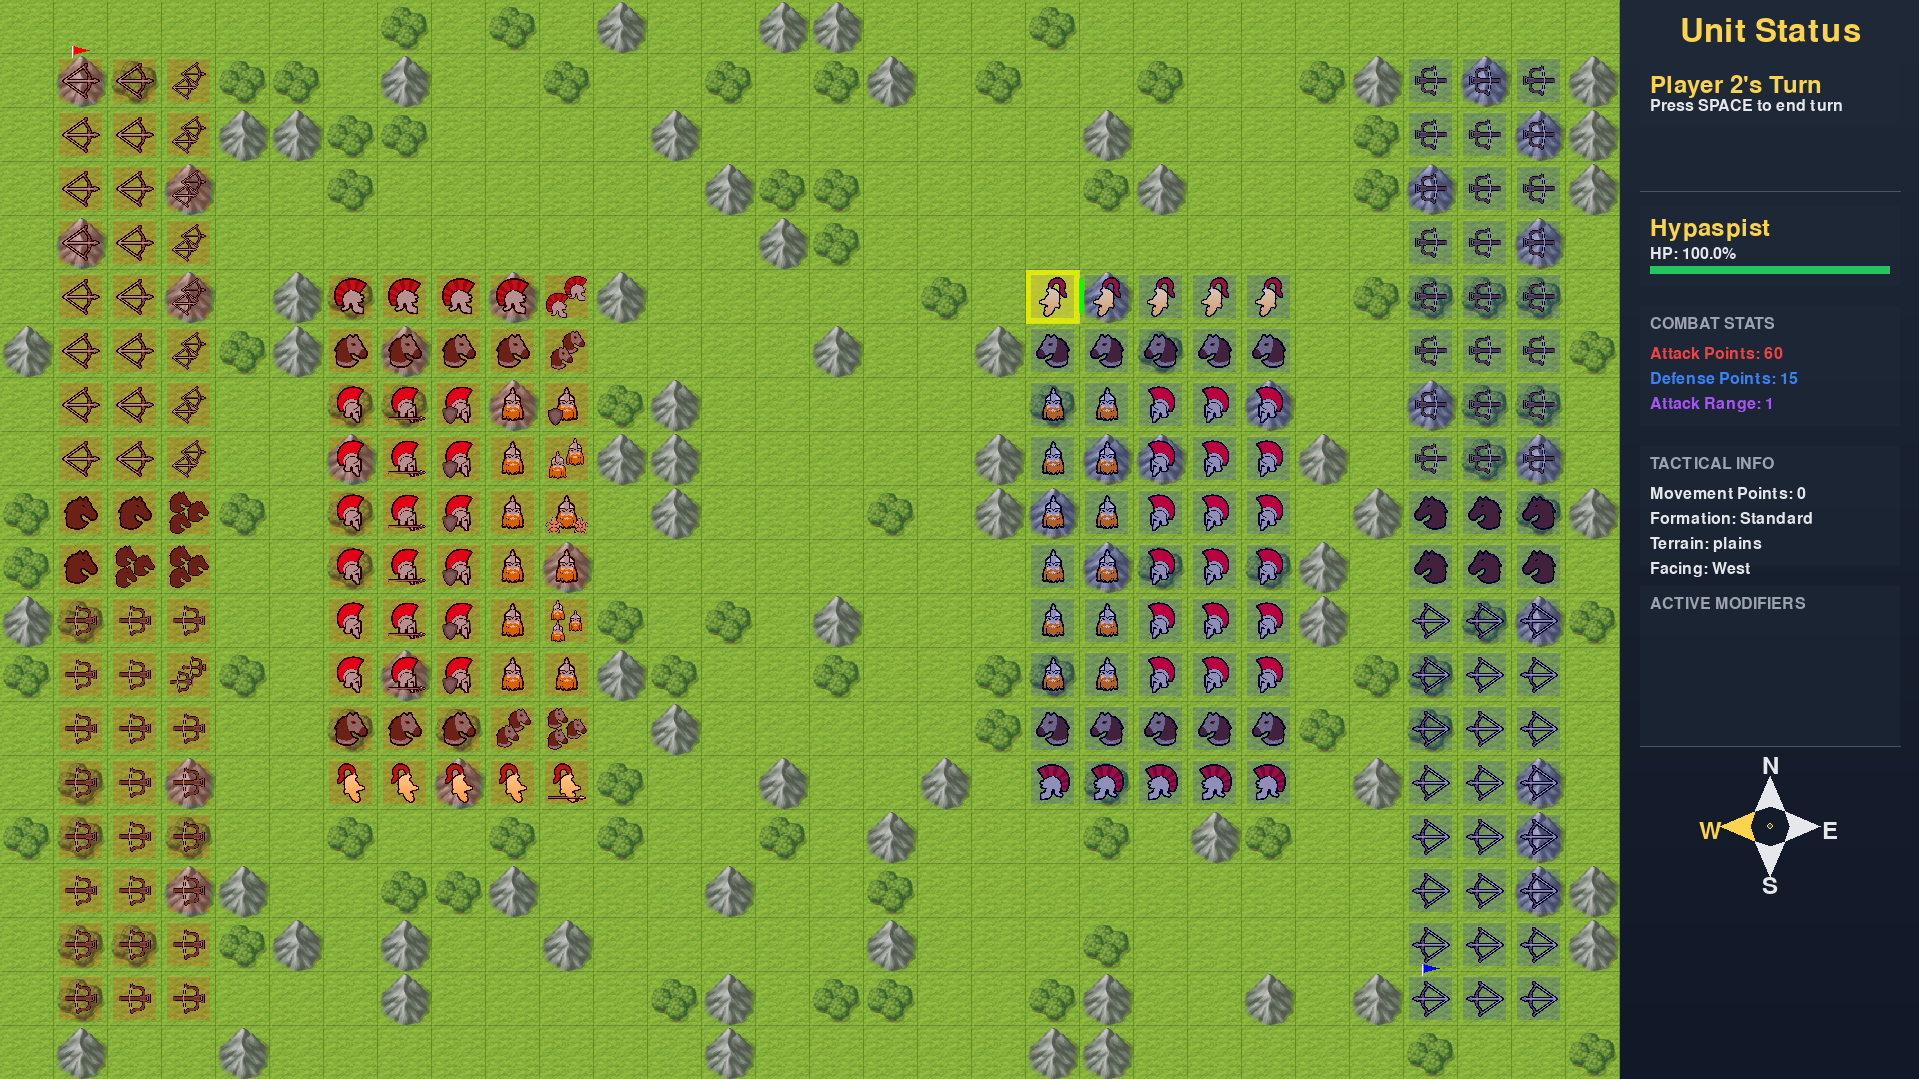
\includegraphics[width=1\linewidth]{figuras/game.png}
    \caption{Warbound}
    \label{fig:game}
\end{figure}

\subsection{Units}

In the initial development of the game, the idea of representing the units using detailed full-body sprites was considered. However, this approach had many challenges, particularly due to the density of units that a single piece could represent on the board. Representing multiple units with a single icon would complicate visualization. Additionally, in one of the versions of the game, it was necessary to increase the size of the board, which would result in excessively small icons, negatively affecting the visual experience of the game.

To overcome these design challenges, a simplified and functional visual style was adopted, with sprites specially adjusted for the game, aligning them with the theme and design of \textit{Warbound}. Additionally, new sprites were created, specifically configured to reflect the different tactical formations available in \textit{Warbound}, allowing players to distinguish between formations during the game.

The units in \textit{Warbound} are categorized into two main types: Melee and Ranged. Each unit is represented by distinct icons that clearly illustrate its role and combat style, making it easy for players to quickly identify the units in play.

The possible units in the game are shown in the figure set below.

\begin{figure}[H]
    \centering
    % Line 1
    \begin{minipage}{0.12\textwidth}
        \centering
        
\includegraphics[width=\textwidth]{figuras/units/hoplite/hoplite.png}
        \caption{Hoplite}
    \end{minipage}\hspace{0.03\textwidth} % Adjusted space
    \begin{minipage}{0.12\textwidth}
        \centering
        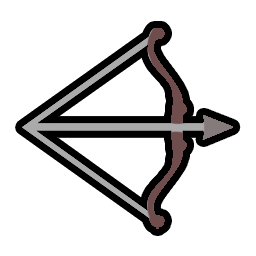
\includegraphics[width=\textwidth]{figuras/units/archer/archer.png}
        \caption{Archer}
    \end{minipage}\hspace{0.03\textwidth} % Adjusted space
    \begin{minipage}{0.12\textwidth}
        \centering
        
\includegraphics[width=\textwidth]{figuras/units/cavalry/cavalry.png}
        \caption{Cavalry}
    \end{minipage}\hspace{0.03\textwidth} % Adjusted space
    \begin{minipage}{0.12\textwidth}
        \centering
        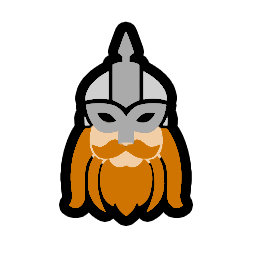
\includegraphics[width=\textwidth]{figuras/units/viking/viking.png}
        \caption{Viking}
    \end{minipage}

    \vspace{0.5cm}

    \begin{minipage}{0.12\textwidth}
        \centering
        
\includegraphics[width=\textwidth]{figuras/units/hypaspist/hypaspist.png}
        \caption{Hypaspist}
    \end{minipage}\hspace{0.03\textwidth}
    \begin{minipage}{0.12\textwidth}
        \centering
        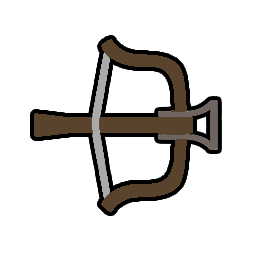
\includegraphics[width=\textwidth]{figuras/units/crossbowman/crossbowman.png}
        \caption{Crossbowman}
    \end{minipage}\hspace{0.03\textwidth} 
    \begin{minipage}{0.12\textwidth}
        \centering
        
\includegraphics[width=\textwidth]{figuras/units/heavy_cavalry/heavy_cavalry.png}
        \caption{Heavy Cavalry}
    \end{minipage}\hspace{0.03\textwidth}
    \begin{minipage}{0.12\textwidth}
        \centering
        
\includegraphics[width=\textwidth]{figuras/units/legionary/legionary.png}
        \caption{Legionary}
    \end{minipage}\hspace{0.03\textwidth}
    \begin{minipage}{0.12\textwidth}
        \centering
        
\includegraphics[width=\textwidth]{figuras/units/men-at-arms/menatarms.png}
        \caption{Men-at-arms}
    \end{minipage}
\end{figure}

\subsection{Formations}

Formations are an important aspect in \textit{Warbound}, offering players the ability to adapt their tactics based on the battle situation. Each formation was designed in a standardized manner to reflect its strategic purpose, influencing the defense, attack, and movement of units. The available formations are shown in the figure set below:

\begin{figure}[H]
    \centering
    \begin{minipage}{0.1\textwidth}
        \centering
        
\includegraphics[width=\textwidth]{figuras/units/hoplite/hoplite.png}
        \caption{Standard}
    \end{minipage}\hspace{0.03\textwidth}
    \begin{minipage}{0.12\textwidth}
        \centering
        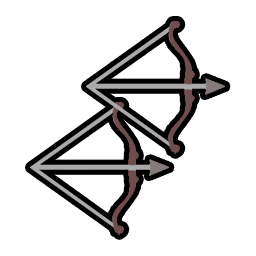
\includegraphics[width=\textwidth]{figuras/units/archer/archer_spread.png}
        \caption{Spread}
    \end{minipage}\hspace{0.03\textwidth}
    \begin{minipage}{0.12\textwidth}
        \centering
        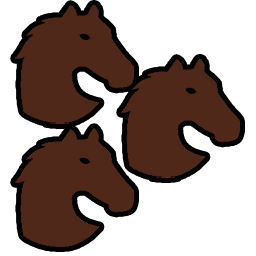
\includegraphics[width=\textwidth]{figuras/units/cavalry/cavalry_V.png}
        \caption{V}
    \end{minipage}\hspace{0.03\textwidth}
    \begin{minipage}{0.12\textwidth}
        \centering
        
\includegraphics[width=\textwidth]{figuras/units/viking/viking_shield_wall.png}
        \caption{Shield Wall}
    \end{minipage}\hspace{0.03\textwidth}
    \begin{minipage}{0.12\textwidth}
        \centering
        
\includegraphics[width=\textwidth]{figuras/units/hypaspist/hypaspist_phalanx.png}
        \caption{Phalanx}
    \end{minipage}\hspace{0.03\textwidth}
    \begin{minipage}{0.12\textwidth}
        \centering
        
\includegraphics[width=\textwidth]{figuras/units/legionary/legionary_turtle.png}
        \caption{Turtle}
    \end{minipage}
\end{figure}

\subsection{Terrains}

The terrain in \textit{Warbound} directly affects the strategy and movement of units. Different types of terrain, such as plains, forests, and mountains, are visually distinct and provide strategic advantages and disadvantages. Below are the designs for each of the available terrains.

\begin{figure}[H]
    \centering
    \begin{minipage}{0.1\textwidth}
        \centering
        
\includegraphics[width=\textwidth]{figuras/terrains/plains.png}
        \caption{Plains}
    \end{minipage}\hspace{0.03\textwidth}
    \begin{minipage}{0.12\textwidth}
        \centering
        
\includegraphics[width=\textwidth]{figuras/terrains/forest.png}
        \caption{Forest}
    \end{minipage}\hspace{0.03\textwidth}
    \begin{minipage}{0.12\textwidth}
        \centering
        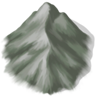
\includegraphics[width=\textwidth]{figuras/terrains/mountain.png}
        \caption{Mountain}
    \end{minipage}
\end{figure}
